% This file is part of the stream_information project.
% Copyright 2017 the authors. All rights reserved.

% # style notes
% - it is Cram\'er--Rao not Cram\'er-Rao. And yet Fisher-matrix not Fisher--matrix.

\documentclass[modern]{aastex61}

% typography
\setlength{\parindent}{1.\baselineskip}
\newcommand{\acronym}[1]{{\small{#1}}}
\newcommand{\CRLB}{\acronym{CRLB}}

% aastex parameters
%%\hypersetup{linkcolor=red,citecolor=green,filecolor=cyan,urlcolor=magenta}
\received{not yet; THIS IS A DRAFT}
%\revised{not yet}
%\accepted{not yet}
%% Adds "Submitted to " the arguement.
%\submitjournal{ApJ}
\shorttitle{information in stellar streams}
\shortauthors{bonaca et al.}

\begin{document}\sloppy\sloppypar\raggedbottom\frenchspacing % trust me

\title{The information content in cold stellar streams}

\correspondingauthor{Ana Bonaca}
% \email{whatevs}

\author[0000-0002-7846-9787]{Ana Bonaca}
\affil{Harvard--Smithsonian Center for Astrophysics}

\author[0000-0003-2866-9403]{David W. Hogg}
\affiliation{Center for Cosmology and Particle Physics,
Department of Physics,
New York University}
\affiliation{Center for Data Science,
New York University}
\affiliation{Flatiron Institute, Simons Foundation}
\affiliation{Max-Planck-Institut f\"ur Astronomie, Heidelberg}

\begin{abstract}\noindent % trust me
Cold stellar streams---produced by tidal disruptions of globular
clusters (or equivalent)---are long-lived, coherent dynamical features
in the stellar halo of the Milky Way.
They have delivered precise information about the mass distribution or
gravitational potential, including constraints on the shape of the
dark-matter halo.
Because of their different positions in phase space, different ages,
and different levels of observational scrutiny, different streams tell
us different things about the Galaxy.
Here we employ a Cram\'er--Rao (\CRLB) or Fisher-matrix approach to
understand the quantitative information content in the known
streams (Pal5, GD-1, Styx, [full list here]).
This approach depends on the existence of a generative model of
stellar streams, which we have developed previously, and which permits
easy calculation of derivatives of predicted stream properties with
respect to Galaxy model parameters.
We find that, in simple, static, analytic models of the Milky Way,
streams XX and YY contain the most information about the dark-matter
shape.
For any individual stream, there are near-degeneracies between
dark-matter halo properties and other parameters, including the mass
of the Large Magellanic Cloud, the total dark-matter mass, and other
potential parameters, but we find that simultaneous fitting of multiple
streams ought to precisely constrain all parameters well.
The \CRLB\ on any one parameter depends strongly on the model freedom;
as we permit more potential freedom, the information about, say, halo
triaxiality, reduces.
We perform experiments to demonstrate this using potential basis
functions that permit great freedom in the gravitational potential on intermediate
scales.
The \CRLB\ formalism also permits us to assess the value of future
measurements of stellar velocities, distances, and proper motions. We
make some comments about the information value of various new
observations that could be made of particular known streams.
\end{abstract}

\keywords{foo --- bar --- hello --- world}

\section{Introduction} \label{sec:intro}

\begin{itemize}
 \item establish streams useful in constraining gravitational potential
 \item tied to parametric models (too complex for inference otherwise, at least in current approaches)
 \item constraints only as good as the model (VL2 results)
 \item so, since not likely that the true potential is NFW, what are the streams constraining? 
 \item here we're building a framework to measure the information content of stellar streams regarding the gravitational potential
 \item two-fold goals: given a simple parametric model, what kind of data do we need? what aspect of a (non-parametric) potential do individual streams constrain?
\end{itemize}


\section{Methods}
\label{sec:method}

\subsection{Information content in stellar streams}
Numerous methods have been developed to estimate properties of a dark matter halo by modeling observations of stellar streams \citep[e.g.,][]{}.
In this approach, the dark matter halo is usually described by an analytic model with a handful of free parameters.
We define the information content in this context as the best-case uncertainties on our model parameters achievable using the observational data at hand.
Formally, the lower bound on the variance of a deterministic parameter is given by the Cram\' er--Rao lower bound \citep[\CRLB][]{Cramer1946, Rao1945}.

For some data set $\vec{y}$ (e.g., a vector of position and velocity measurements of stars along a stream), the associated covariance matrix is $C_y$.
Given the model parameters $\vec{x}$ (e.g., a vector with the mass and scale radius of a dark matter halo), the Cram\' er--Rao bound is given by the covariance matrix $C_x$.
The \CRLB\ is set by the inverse of a Fisher information matrix \citep{}:
\begin{equation}
C_x^{-1} = \left(\frac{d\vec{y}}{d\vec{x}}\right)^{T} C_y^{-1} \left(\frac{d\vec{y}}{d\vec{x}}\right)
\label{eq:crlb}
\end{equation}
In the next two subsections, we describe individual terms of Equation~\ref{eq:crlb}: the change in stream observables $\vec{y}$ as a function of changes in the gravitational potential $\vec{x}$, i.e., the derivative $d\vec{y}/d\vec{x}$, in \S\ref{sec:derivatives}, and the adopted observational uncertainties, which set the covariance matrix $C_y$, in \S\ref{sec:datasets}.

\subsection{Calculating numerical derivatives for the \CRLB}
\label{sec:derivatives}
\begin{itemize}
 \item fiducial potential
 \item numerical derivative
 - regard only transverse direction, as longitudinal has a strong degeneracy with stream age
 - rotate to a system of where the equator is a best-fitting great circle to the stream
 - noisy data due to the particle nature of streams, tested time step small enough so that we're not introducing numerical noise that way
 - interested in a general shape of the stream, so we're fitting a bspline to the stream (more stable than polynomial)
 - choice of step size for numerical derivative such that the derivative converged
\end{itemize}

\subsection{Sets of observational data}
\label{sec:datasets}
\begin{itemize}
 \item fiducial
 \item DESI-like
 \item Gaia DR2
 \item MM
 \item SDSS-5
 \item Gaia final
\end{itemize}

\subsection{Cold tidal streams in the Milky Way}


\section{Results}



\begin{figure}
\begin{center}
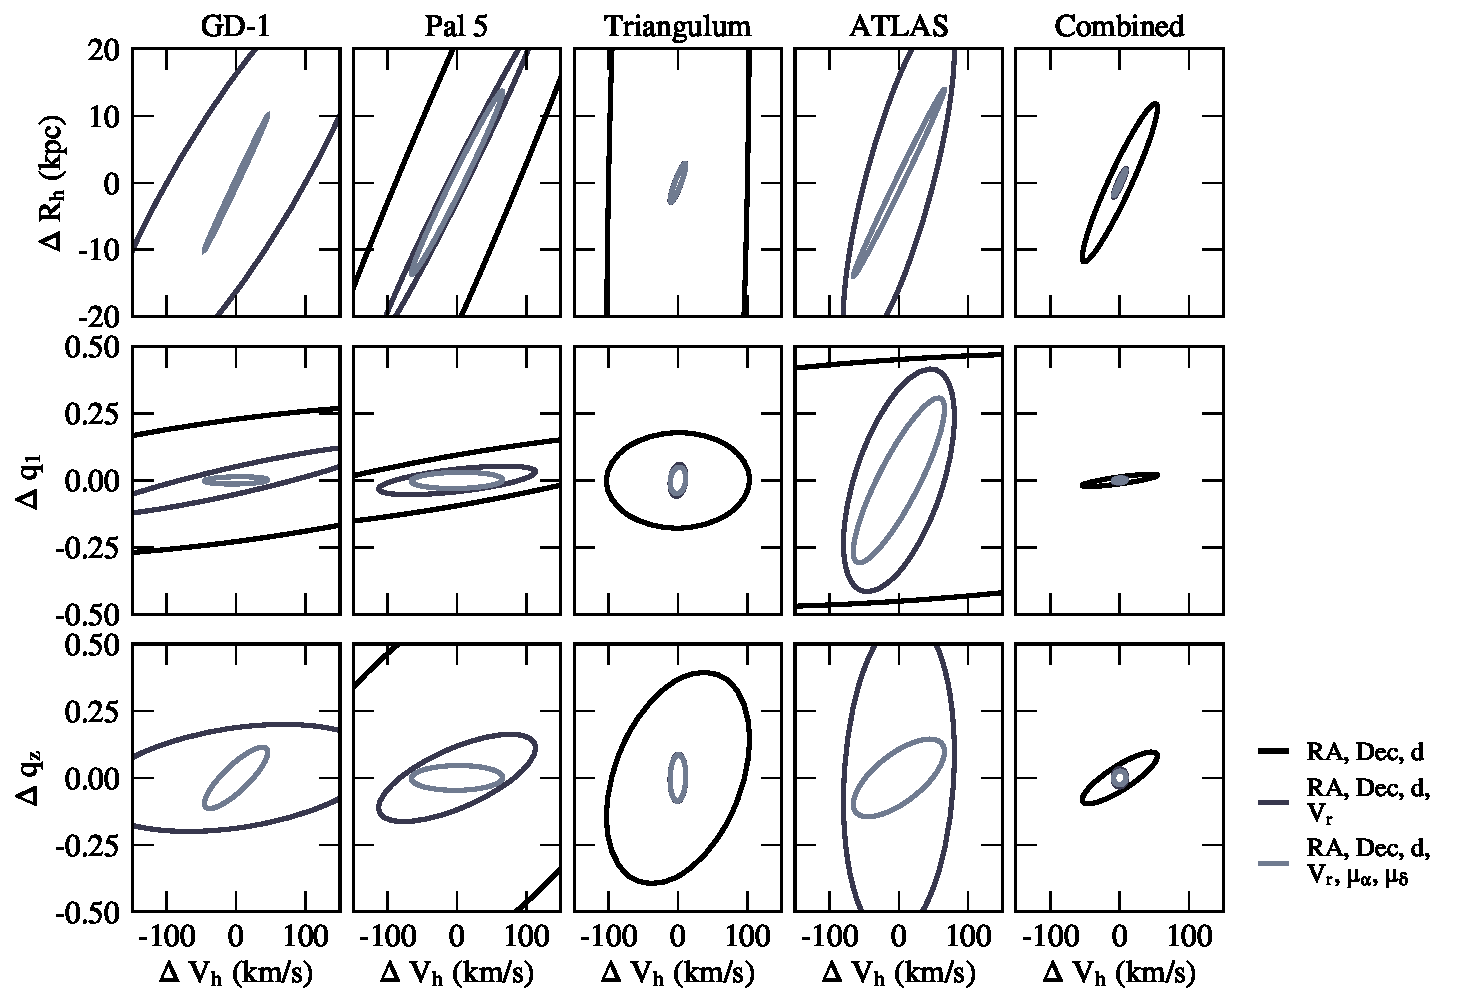
\includegraphics[width=\textwidth]{crlb_2d.pdf}
\caption{Two-dimensional Cram\' er--Rao lower bounds that cold stellar streams put on parameters of the Milky Way dark matter halo.
Parameters considered are the halo scale velocity $V_h$, scale radius $R_h$, $x/y$ and $z/y$ axis ratios $q_1$ and $q_z$, respectively.
Parameter combination is the same across the rows.
Bounds based on individual streams (GD-1, Pal~5, Triangulum and ATLAS) are shown in the first four columns, and their combination is presented in the last column.
The ellipse color denotes the dimensionality of the observational data used to calculate the bound; the darkest ellipses are based on positional information only, medium-colored ellipses include positions and radial velocity, and the lightest ellipses are derived using the full 6-D phase space of streams.
Not all streams are equally constraining for all of the parameters, but for a given stream, parameter constraints improve when more phase-space dimensions are included.
Combining different streams results in the most precise recovery of the halo parameters.
Even if only limited observational data is available for multiple streams, the obtained bounds are comparable to, or better than, the best bounds coming from any individual stream.
}
\label{fig:2dbounds}
\end{center}
\end{figure}

\bibliographystyle{aasjournal}
\bibliography{crlb}

\end{document}

